\documentclass[twocolumn]{aastex631}

\usepackage{graphicx}
\usepackage{amsmath}
\usepackage{amssymb}
\usepackage{newtxtext,newtxmath}
\usepackage{hyperref}
\usepackage{gensymb}
\usepackage{enumitem}

\newcommand{\vdag}{(v)^\dagger}
\newcommand\aastex{AAS\TeX}
\newcommand\latex{La\TeX}

\newcommand{\Msun}{\ensuremath{M_{\odot}}}
\newcommand{\Gyr}{\ensuremath{\textrm{Gyr}}}
\newcommand{\Myr}{\ensuremath{\textrm{Myr}}}
\newcommand{\yr}{\ensuremath{\textrm{yr}}}
\newcommand{\kpc}{\ensuremath{\textrm{kpc}}}
\newcommand{\ckpc}{\ensuremath{\textrm{ckpc}}}
\newcommand{\pc}{\ensuremath{\textrm{pc}}}
\newcommand{\kms}{\ensuremath{\textrm{km}/\textrm{s}}}
\newcommand{\tocite}{\textcolor{blue}{cite}}
\newcommand{\FeH}{\ensuremath{[\textrm{Fe}/\textrm{H}]}}
\newcommand{\MgFe}{\ensuremath{[\textrm{Mg}/\textrm{Fe}]}}
\newcommand{\OFe}{\ensuremath{[\textrm{O}/\textrm{Fe}]}}
\newcommand{\alphaFe}{\ensuremath{[\alpha/\textrm{Fe}]}}
\newcommand{\tform}{\ensuremath{t_{\textrm{form}}}}
\newcommand{\dex}{\ensuremath{\textrm{dex}}}
\newcommand{\Msunyr}{\ensuremath{\Msun/\textrm{yr}}}
\newcommand{\Atmax}{\ensuremath{A_{2,\textrm{max}}}}

\newcommand{\red}[1]{\textcolor{red}{#1}}

% \received{March 1, 2021}
% \revised{April 1, 2021}
%\accepted{\today}

\shorttitle{Abundance Bimodality in TNG}
\shortauthors{Beane et al.}

\graphicspath{{./}{fig/}}

\begin{document}

\title{Rising from the Ashes II: Can Bar Formation Lead to Abundance Bimodalities?}

\author{Angus Beane}
\affiliation{Center for Astrophysics $|$ Harvard \& Smithsonian, Cambridge, MA, USA}

\author{James W. Johnson}
\affiliation{The Observatories of the Carnegie Institution for Science, Pasadena, CA, USA}

\author{Vadim Semenov}
\affiliation{Center for Astrophysics $|$ Harvard \& Smithsonian, Cambridge, MA, USA}

\author{Lars Hernquist}
\affiliation{Center for Astrophysics $|$ Harvard \& Smithsonian, Cambridge, MA, USA}

\author{Vedant Chandra}
\affiliation{Center for Astrophysics $|$ Harvard \& Smithsonian, Cambridge, MA, USA}

\author{Charlie Conroy}
\affiliation{Center for Astrophysics $|$ Harvard \& Smithsonian, Cambridge, MA, USA}

\begin{abstract}
    The Milky Way is known to host at least two modes in its present day distribution of Fe and $\alpha$-elements. The exact cause of this bimodality is disputed, but one class of explanations involves the merger between the Milky Way and a relatively massive satellite (Gaia-Sausage-Enceladus) at $z\sim2$. However, reproducing this bimodality in simulations is not straightforward, with conflicting results on the prevalance, morphology, and mechanism behind multimodality. We present a case study of a galaxy in the Illustris TNG50 simulation which undergoes a sequence of starburst, brief quiescence, and then rejuvenation. After a minor post-processing step which boosts the \alphaFe{} of old star particles, we demonstrate that this galaxy hosts a strongly bimodal distribution in the \alphaFe{}-\FeH{} plane. The high- and low-$\alpha$ sequences are neatly separated in time by the brief quiescent period. The quiescent period in this galaxy is not associated with a merger but by the formation of a bar followed by AGN activity. This galaxy indicates a novel scenario in which the $\alpha$-bimodality is caused by AGN-induced quenching triggered by the formation of the Milky Way's bar. We argue that the post-processing step can be interpreted as the TNG model underproducing star formation in the densest regions at high-$z$.
  \end{abstract}
    
  \keywords{Classical Novae (251) --- Ultraviolet astronomy(1736) --- History of astronomy(1868) --- Interdisciplinary astronomy(804)}
  

\section{Introduction}\label{sec:intro}
The stellar surface abundances of most elements retain the composition of their natal gas cloud. Therefore, the present-day distribution of stellar surface abundances encodes the chemical history of a galaxy's gas phase. Two elements have received particular interest in the Milky Way: Fe and $\alpha$-elements (elements produced through the $\alpha$-process, such as O and Mg). Fe is produced in both Type Ia and Type II SNe whereas $\alpha$-elements are produced predominantly through Type II SNe. Because these SNe occur on different timescales (10s of Myr after star formation for Type II, as compared to 100s of Myr to Gyrs for Type Ia), the ratio between $\alpha$-elements and Fe is expected to generally decrease with time.

Because of their separate formation channels, the two dimensional plane of \alphaFe{}-\FeH{} has received considerable interest. In the Milky Way, there is a well-established bimodality with separate high- and low-$\alpha$ sequences \citep{1996ASPC...92..307G,1998A&A...338..161F,2004AN....325....3F,2006MNRAS.367.1329R,2011A&A...535L..11A,2012A&A...545A..32A,2014A&A...562A..71B,2014ApJ...796...38N,2020MNRAS.493.2952H}. This bimodal distribution is shown in the upper left panel of Figure~\ref{fig:fig1}.

There are essentially two approaches to explaining the bimodality. First, it is a result of internal secular processes that generate the bimodality through radial migration \citep{2009MNRAS.396..203S,2021MNRAS.507.5882S,2023MNRAS.523.3791C} or clump formation \citep{2019MNRAS.484.3476C,2020MNRAS.492.4716B,2021MNRAS.502..260B,2023ApJ...953..128G}.

Second, the bimodality is generated through gas infall scenarios, either from specific gas accretion episodes from the intergalactic medium \citep{1997ApJ...477..765C,2009IAUS..254..191C,2017MNRAS.472.3637G,2019A&A...623A..60S}, or through a more self-consistent collapse sequence of the circumgalactic medium driven through feedback \citep{2021MNRAS.501.5176K}. Third and finally, the bimodality is generated through a merger process, either by enhancing the SFR of the Galaxy \citep{2004ApJ...612..894B,2005ApJ...630..298B,2007ApJ...658...60B,2010MNRAS.402.1489R} or by supplying a relatively pristine gas supply that resets the metallicity of the Galaxy \citep{2020MNRAS.491.5435B,2024MNRAS.528L.122C}. The fact that the Milky Way did undergo a merger with the Gaia-Sausage-Enceladus (GSE) satellite supports these scenarios \citep{2018MNRAS.478..611B,2018Natur.563...85H,2020ApJ...901...48N,2024ApJ...972..112C}.

In \citet{2024arXiv240707985B} we argued for an alternate formation scenario of the bimodality, for which we provide further support in this work. In this scenario, the bimodality is formed through a brief quiescent period in the Galaxy's history. During this period, which lasted $\sim300\,\Myr$ in that setup, two things happen. First, as the chemical evolution of the galaxy proceeds, fewer stars form. Second, because the SFR is lower, $\alpha$-element production drops and so the \alphaFe{} of the gas drops as well. This is conceptually similar to some variants of the two-phase infall scenarios which allow for a brief halt in the star formation rate \citep[][and references therein]{2024arXiv240511025S}, though the quiescent period is much shorter in \citet{2024arXiv240707985B}. The combination of these two effects is what leads to the valley in between the high- and low-$\alpha$ sequences.

In that work, we used idealized simulations of a galaxy merger that triggered a starburst which preceded the quiescent period. However, we argued that the merger aspect of that work was not necessary, but rather the quiescence. In this work, we study a subhalo from the Illustris TNG50 simulation which demonstrates this. This subhalo of interest (SoI) exhibits the sequence of events presented in \citet{2024arXiv240707985B} after a simple post-processing step which enhances the \alphaFe{} of old star particles. The SoI undergoes a brief quiescent period which neatly separates a high- and low-$\alpha$ sequence. However, instead of being preceded by a merger, the quenching is preceded by apparent bar-induced AGN activity. Therefore, this work serves as a verification that the scenario in \citet{2024arXiv240707985B} is possible in cosmological simulations and can occur in non-merger scenarios.

In Section~\ref{sec:methods} we discuss our selection technique which led to discovering the SoI, the observations we use for comparison, as well as a simple one zone chemical evolution model we use to justify our post-processing step. In Section~\ref{sec:results} we present the main results which we discuss and interpret in Section~\ref{sec:disc}. We conclude in Section~\ref{sec:conc}.

% This decline of \alphaFe{} over time has long been recognized \citep{1979ApJ...229.1046T}. This trend is only generally true, though, with non-monotonic behavior observed in observations and even one-zone chemical models \citep[e.g.][]{2022arXiv220402989C}. 

\section{Methods}\label{sec:methods}
\subsection{IllustrisTNG Sample}\label{ssec:tng}
We have made use of the Illustris TNG50 simulation \citep{2019MNRAS.490.3196P, 2019MNRAS.490.3234N}, a cosmological simulation of a $\sim50\,\textrm{cMpc}$ box at high resolution ($m_{\textrm{baryon}}\sim8.5\times10^4\,\Msun$). It uses the gravito-magneto-hydrodynamics code \texttt{AREPO} \citep{2010MNRAS.401..791S, 2016MNRAS.455.1134P}, along with the TNG model \citep{2013MNRAS.436.3031V, 2017MNRAS.465.3291W, 2018MNRAS.473.4077P}. This model includes several subgrid processes: a wind generation model, chemical enrichment from supernovae and asymptotic giant branch stars, and thermal and kinetic feedback from AGN.

One piece of the TNG model of note for this work is the BH accretion and feedback method \citep{2017MNRAS.465.3291W}. The black hole accretion rate ($\dot{M_{\textrm{BH}}}$) is computed using the local structure of the gas phase with the Bondi-Hoyle-Lyttleton formula \citep{1939PCPS...35..405H,1944MNRAS.104..273B,1952MNRAS.112..195B}, with a maximum of the Eddington accretion rate ($\dot{M_{\textrm{edd}}}$). The model allows the BH to be either in a kinetic radio-mode or a thermal quasar-mode. If the Eddington ratio ($\dot{M_{\textrm{BH}}}/\dot{M_{\textrm{edd}}}$) exceeds a threshold ($M_{\textrm{BH}}$-dependent, but $\sim0.001--0.1$), the BH is in the quasar mode and injects a large amount of thermal energy into its surroundings.

Using the public catalog, we selected a sample of subhalos at $z=1.5$ (snapshot 40) according to the following criteria: (1) the subhalo is central (i.e., the most massive subhalo within its halo), and (2) the subhalo's stellar mass is between $10^{10}$ and $10^{10.5}\,\Msun/\textrm{h}$. There were a total of 168 subhalos that met both criteria. The chosen mass range is broadly consistent with the expected mass of the Milky Way at this redshift \citep{2013ApJ...771L..35V}. We chose to make our selection of galaxies at $z=1.5$ instead of at lower redshift because we wished to capture the \textit{formation} of any multimodal structure. We did not want contamination by mergers at lower redshift which we know contribute very little to the Milky Way's disk stars \citep[e.g.,][]{2016ARA&A..54..529B}.

We examined the abundance distribution in the \MgFe{}-\FeH{} plane of this sample of subhalos by eye. Not many subhalos had multimodal structure, and any structure that was present was relatively weak compared to that observed in the Milky Way. We then applied a post-processing to the \MgFe{} of stars by adding to each star particle a value of $0.1\times\left(t_{1.5}-t_{\textrm{form}}\right)$, where $t_{1.5}$ is the age of the universe at $z=1.5$ ($\sim4.3\,\Gyr$) and $t_{\textrm{form}}$ is the formation time of each star particle. With this post-processing, we found that much more structure was generally present.

We show the abundance distributions (replicating Figure~\ref{fig:fig1}) of 16 random subhalos from our catalog, and the subhalo we selected, in Appendix~\ref{app:rand_fig1}. Of these subhalos, some structure is present, but none have a strong bimodality as seen in the Milky Way. After the $\alpha$-enhancement, a few have strongly bimodal features (subject to interpretation): 172175, 178140, 193025.

We selected subhalo 172175 (the ID at snapshot 40) for its particular resemblance to the Milky Way. We then studied the main descendant of this subhalo at $z=0$ (subhalo 392276 at snapshot 99). We refer to this subhalo as our subhalo of interest (SoI).

\subsection{Bar Catalog}\label{ssec:barcat}
In order to study the evolution of the morphology of our SoI, we make use of the \citet{2022MNRAS.515.1524Z} catalog. They provide a decomposition of all galaxies with at least $10^4$ star particles, as well as an estimate of the bar strength. This taken to be the maximum of the second Fourier mode ($A_{2,\textrm{max}}$) within the bar region (not including spiral arms).

\subsection{Observations}\label{ssec:obs}
We make use of two observational data sets. First, we use the ASPCAP DR17 catalog of stellar abundances \citep[][J.A.~Holtzman et al., in preparation]{2016AJ....151..144G}. We make the same selection cuts as in \citet{2024arXiv240707985B}, described in their Section~2.4. These are meant to select only giants with high quality abundance measurements as well as restricting the sample to only stars in the disk with angular momenta similar to the Sun's. This results in a sample of 54,777 stars. We use Fe to track total metallicity and Mg alone as an $\alpha$-element.

We then further considered a dataset of stellar ages from the APOKASC2 catalog \citep{2018ApJS..239...32P}. This uses a combination of APOGEE spectroscopic parameters and \textit{Kepler} time series photometry to compute astroseismic ages. Using only stars with $25\%$ age uncertainties (taken as the maximum of the upper and lower uncertainty), we cross-match this catalog to our larger sample from ASPCAP which results in a sample of 1201 stars.

\subsection{One-Zone Chemical Evolution Model}\label{ssec:onezone_met}
James inserts his section

\section{Results}\label{sec:results}
\subsection{Abundance Plane}\label{ssec:plane}

\begin{figure*}
  \centering
  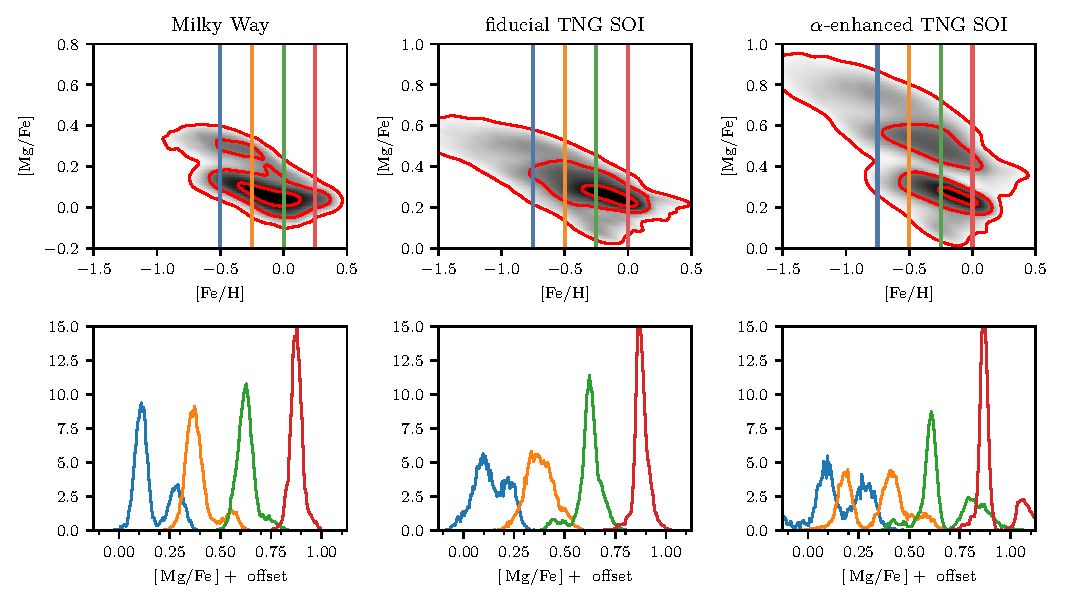
\includegraphics[width=\textwidth]{fig/392276.pdf}
  \caption{\textbf{When old stars are $\alpha$-enhanced, our subhalo of interest from TNG displays a prominent bimodality.} The upper left panel shows the distribution in the \MgFe{}-\FeH{} plane of the Milky Way, demonstrating a clear bimodality (data selection given in text). The lower left panel shows the 1D histograms of \MgFe{} at fixed \FeH{} values of $-0.5$, $-0.25$, $0$, and $0.25$ (blue, orange, green, and red, respectively). In the Milky Way, the bimodality is strongest at low metallicities while disappearing at high metallicities. The middle column shows the same plots but for our TNG subhalo of interest (392276) and with the fixed \FeH{} values $0.25\,\dex$ lower. Only faint structure is seen in the lowest bin (blue, $-0.75\,\dex$). The right column shows the same subhalo but after increasing the \MgFe{} value of star particles formed before $z=1.5$ linearly with formation time (specifically by incrementing \MgFe{} by $0.1\times\left(t_{1.5}-t_{\textrm{form}}\right)$ if $t_{\textrm{form}} < t_{1.5}$, where $t_{1.5}$ is the age of the universe at $z=1.5$). A clear bimodality is shown in these panels which, unlike in the Milky Way, is present at all metallicities.}
  \label{fig:fig1}
\end{figure*}

The main result of our paper is given in Figure~\ref{fig:fig1}. Here, we compare the abundance plane in the Milky Way (left column) to that in our subhalo of interest (middle and right columns). The upper panels show the 2D distribution in the space of \MgFe{}-\FeH{}. We have applied the standard \texttt{scipy} implementation of a gaussian kernel density estimator to a Cartesian grid of points. For each panel, we normalize so that the integral of the distribution is unity. Colors are plotted in a log scale ranging from $0.08$ to $15\,\dex^{-2}$. Contour lines are plotted at $0.1$, $1.5$, and $10\,\dex^{-2}$.

The colored vertical lines are indicated at $\FeH=-0.75$, $-0.5$, $-0.25$, and $0\,\dex$ in the Milky Way, and at bins $0.25\,\dex$ higher in the simulations. The lower panels show 1D histograms of \MgFe{} in bins centered on these values. The bins for the Milky Way/simulations have width $0.2$/$0.05\,\dex$. The \MgFe{} values are given offsets so their medians are at zero. The rationale for the higher plotted \FeH{} in the simulations comes just from the empirical location of the bimodalities. The Milky Way shows a clear bimodal population, with a high-$\alpha$ sequence most clearly distinct from the low-$\alpha$ sequence at low metallicity. The two sequences merge around solar metallicity.

Our SoI, on the other hand, does not show a clearly bimodal structure in the fiducial simulation (middle column). There is some structure in the $\FeH=-0.75$ bin. The right panel of Figure~\ref{fig:fig1} shows the same distribution as in the middle panel, but with a post-processed declination in \MgFe{} described in Section~\ref{ssec:tng}. Star particles formed before $z=1.5$ are given an additive offset of $0.1\times\left(t_{1.5}-t_{\textrm{form}}\right)$, where $t_{1.5}$ is the age of the universe at $z=1.5$ and $t_{\textrm{form}}$ is the formation time of the star particle. A multimodal structure emerges with three clear modes at $\MgFe\sim0.8$, $0.5$, and $0.2\,\dex$. The 1D histograms show that the modes are well-separated, and that the troughs between the modes nearly vanish.

\subsection{Alpha Time Dependence}\label{ssec:alpha_time}

\begin{figure*}
  \centering
  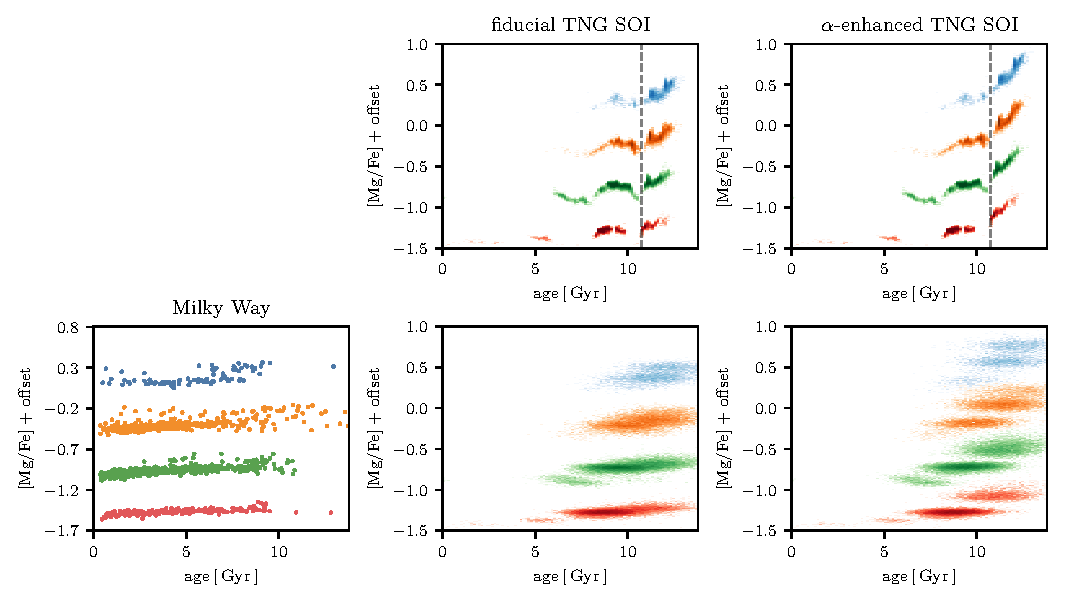
\includegraphics[width=\textwidth]{fig/392276_alpha.pdf}
  \caption{\textbf{Bimodality in the abundance plane is linked to distinct epochs in simulation.} The upper panels show \MgFe{} as a function of age for our subhalo in TNG. The colors indicate stellar populations at fixed values of \FeH{}, which are the same as in Figure~\ref{fig:fig1}. A gap in the relation occurs at an age of approximately $10.6\,\Gyr$, which we indicate with a vertical dashed line. The effect of the $\alpha$-enhancement is clear, as it separates the stars that form before and after this gap in ages (star particles which formed before $z=1.5$ are $\alpha$-enhanced, which occurs at an age of $\sim9.5\,\Gyr$). The lower panels show on the left the Milky Way and on the center and right the data from TNG but with $15\%$ age errors and $0.01\,\dex$ errors in \MgFe{}. When the simulations are given these errors, we see that the before and after star particles smear such that the two populations significantly overlap in ages. In the $\alpha$-enhanced SoI, two populations emerge in each bin which overlapped in the fiducial distribution. This feature more closely resembles the Milky Way, which displays such populations where the bimodality is strongest -- $\FeH=-0.5$ (blue) and $-0.25$ (orange).}
  \label{fig:alpha}
\end{figure*}

The abundance distributions shown in Figure~\ref{fig:fig1} can be better understood by examining the evolution of \MgFe{} with time of the individual stars/star particles. In the upper panels of Figure~\ref{fig:alpha} we show the true distribution of \MgFe{} as a function of time for the fiducial SoI in the middle and for the post-processed, $\alpha$-enhanced subhalo to the right. We use age instead of formation time in order to better facilitate comparisons to observations. These panels are true 2D histograms, with a logarithmic colormap normalized to the maximum of the plot. The values of \MgFe{} are offset so their medians are at zero.

There is a gap in the ages that occurs at an age of $10.6\,\Gyr$, which we mark with a vertical dashed line. Star particles older than this line have a much clearer gradient in time with \MgFe{} than stars that form after. In the $\FeH=-0.25$ bin, star particles which form directly after this line have a slightly depressed \MgFe{} than stars which form a short time later.

In the lower panels we plot to the left data from the Milky Way and to the middle and right from the fiducial and $\alpha$-enhanced SoI, respectively. For the simulations, we add $15\%$ age and $0.01\,\dex$ \MgFe{} Gaussian errors. These values are roughly in line with the observational errors from the APOKASC2 and APOGEE datasets that the lower left panel is made from (see Appendix~\ref{app:obs_err} for plots of the observational errors). The error in \MgFe{} is not signficant, but the age error, which is $1.5\,\Gyr$ at $10\,\Gyr$, smears out the distribution before and after the dashed line. The $\alpha$-enhanced SoI still shows two separate populations in this plot, but they now significantly overlap in age.

The Milky Way distribution (lower left panel) bears some resemblance to the $\alpha$-enhanced SoI. In particular, the $\FeH=-0.5$ and $-0.25$ bins (blue and orange, respectively) show what appears to be two populations overlapping in age but nonetheless separated in \MgFe{}. These are the bins at which the bimodality is strongest (upper left panel of Figure~\ref{fig:fig1}).

\subsection{Evolutionary History}\label{ssec:evol}

\begin{figure}
  \centering
  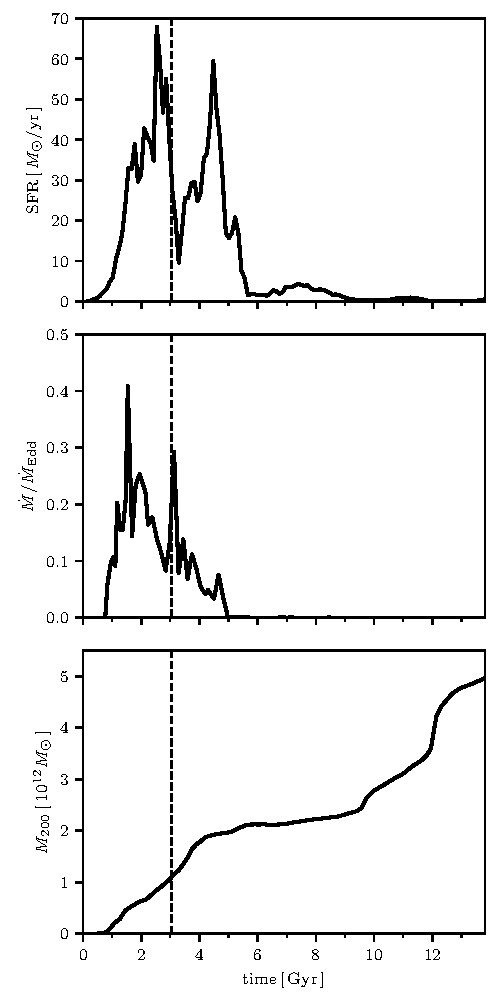
\includegraphics[width=\columnwidth]{fig/392276_SFH_AGN_M200.pdf}
  \caption{\textbf{The evolutionary history of our subhalo of interest.} The upper panel shows the SFH of our subhalo. This SFH is computed using the SFR within twice the stellar half-mass radius in our SoI's main progenitors. In this and all subsequent panels we show a vertical dashed line at the same position as in Figure~\ref{fig:alpha} ($\sim3.2\,\Gyr$), which delineates the separation between the high- and low-$\alpha$ sequences. The gap in ages is naturally associated with a gap in the SFH located at the dashed line. The middle panel shows the BH accretion rate as a fraction of the maximum (Eddington) accretion rate across time. The accretion rate is high early on, but then drops. The gap in ages (dashed line) is coincident with a local peak in the BH accretion rate. In the lower panel we show the mass assembly of the halo, given as the mass within the radius that encloses $200\times$ the mean density of the universe. In this plot mergers are shown as sudden increases in $M_{200}$. Mergers at very early times when the halo is signifcantly less massive than its $z=0$ mass are not shown, but one can see that no clear merger is associated with the gap in stellar ages. Two mergers occur later on at $t\sim10$ and $\sim12\,\Gyr$.}
  \label{fig:history}
\end{figure}

In an effort towards understanding the events in our SoI's history that led to the behavior around the dashed line in Figure~\ref{fig:alpha}, we examine the evolution of some of its key quantities. In the upper panel of Figure~\ref{fig:history}, we show the SFH of our galaxy with the same dashed line as in Figure~\ref{fig:alpha} (at an age of $10.6\,\Gyr$ in that plot is at a time of $\sim3.2\,\Gyr$ here). This SFH is computed using the SFR within twice the stellar half-mass radius in our SoI's main progenitors. We see two peaks in the SFH at $t\sim2.5$ and $\sim4.5\,\Gyr$ of an amplitude of about $50$ and $30\,\Msunyr$. The dashed line corresponds to a relative drop in the SFR, down to about $3\,\Msunyr$ before quickly recovering.

The middle panel shows the accretion rate of the central black hole as a fraction of the maximum (Eddington) accretion rate. Early in its history ($t<2\,\Gyr$), the subhalo experiences high accretion rates. The accretion rate then steadily declines until $t\sim5\,\Gyr$ at which point it fails to show on this linear plot. However, at the dashed line ($\sim3.2\,\Gyr$) there is a localized peak in the accretion rate, maxing out at about $30\%$ Eddington. This places the BH firmly in the thermal quasar-mode, and allows it to inject large amounts of thermal energy into the center of the galaxy.

The lower panel shows the virial mass of the subhalo, as measured by $M_{200}$ -- the mass within the radius that encloses a region of density $200\times$ the mean density of the universe. Early on at $t<4\,\Gyr$ the virial mass grows roughly linearly up to $\sim2\times10^{12}\,\Msun$. After that, the virial mass remains roughly constant until sharp increases at $t\sim10$ and $\sim12\,\Gyr$. The transition in the virial mass from linear to constant at $t\sim4\,\Gyr$ is followed $1\,\Gyr$ later by a sudden drop in the SFR and BH accretion rate.

\begin{figure}
  \centering
  \includegraphics[width=\columnwidth]{fig/392276_SFH_AGN_M200_zoomed.pdf}
  \caption{\textbf{At the transition from the high- to low-$\alpha$ sequence, a bar forms and strengthens, AGN activity is enhanced, and star formation is supressed.} The evolutionary history of our SoI near the transition between the high- and low-$\alpha$ sequence, which is indicated as a vertical dashed line at an age of $10.6\,\Gyr$ ($t\sim3.2\,\Gyr$). The blue line indicates the SFR, which drops from a peak of $\sim54\,\Msunyr$ to $\sim3.6\,\Msunyr$. The minimum is very close to the transition. The drop in SFR is coincident with a rise in the AGN accretion rate (orange) as well as a rise in the strength of the bar (red).}
  \label{fig:history_zoom}
\end{figure}

We show the evolution of the SoI in greater detail at the transition between the high- and low-$\alpha$ sequences in Figure~\ref{fig:history_zoom}. As in Figure~\ref{fig:history}, we indicate the SFR (blue) and black hole accretion rate (orange), but we also include the strength of the bar, taken to be the maximum value of $A_2$ in the bar region, in red. From $\sim2.8\,\Gyr$ to $\sim3.2\,\Gyr$, the SFR drops from $\sim54$ to $3.6\,\Msunyr$. The minimum in the SFR is nearly coincident with the transition line.

We can see more clearly here that the BH accretion rate (red), in units of the Eddington accretion rate, increases from a value of $\sim0.08$ at $\sim2.8\,\Gyr$ to a maximum of $\sim0.3$ at $\sim3.1\,\Gyr$, right before the transition. This rise in the AGN accretion rate is preceded by a strengthening of the bar, which rises from an $A_2$ of $\sim0.1$ at $t\sim2.4\,\Gyr$ to an $A_2$ of $\sim0.5$ at $\sim3.1\,\Gyr$, the time of the peak BH accretion rate.

\subsection{Images}\label{ssec:images}
\begin{figure*}
  \centering
  \includegraphics[width=\textwidth]{fig/images_star.pdf}
  \caption{Surface density projections of star particles in our SoI at the transition between the high- and low-$\alpha$ sequences. Each panel indicates subsequent snapshots ranging from snapshot 23 ($z\sim3.5$) to snapshot 36 ($z\sim1.7$), as well as snapshot 99 ($z=0$) in the lower right. Several key numbers are shown in the corners of each panel, clockwise from the top left: SFR, time, bar strength ($A_{2,\textrm{max}}$), and BH accretion rate. A guide is given in the top left subpanel. At the center-bottom of each panel, we indicate panels which occur before the transition ($\sim3.2\,\Gyr$) as high-$\alpha$ and panels which occur after as low-$\alpha$.}
  \label{fig:images_star}
\end{figure*}

\begin{figure*}
  \centering
  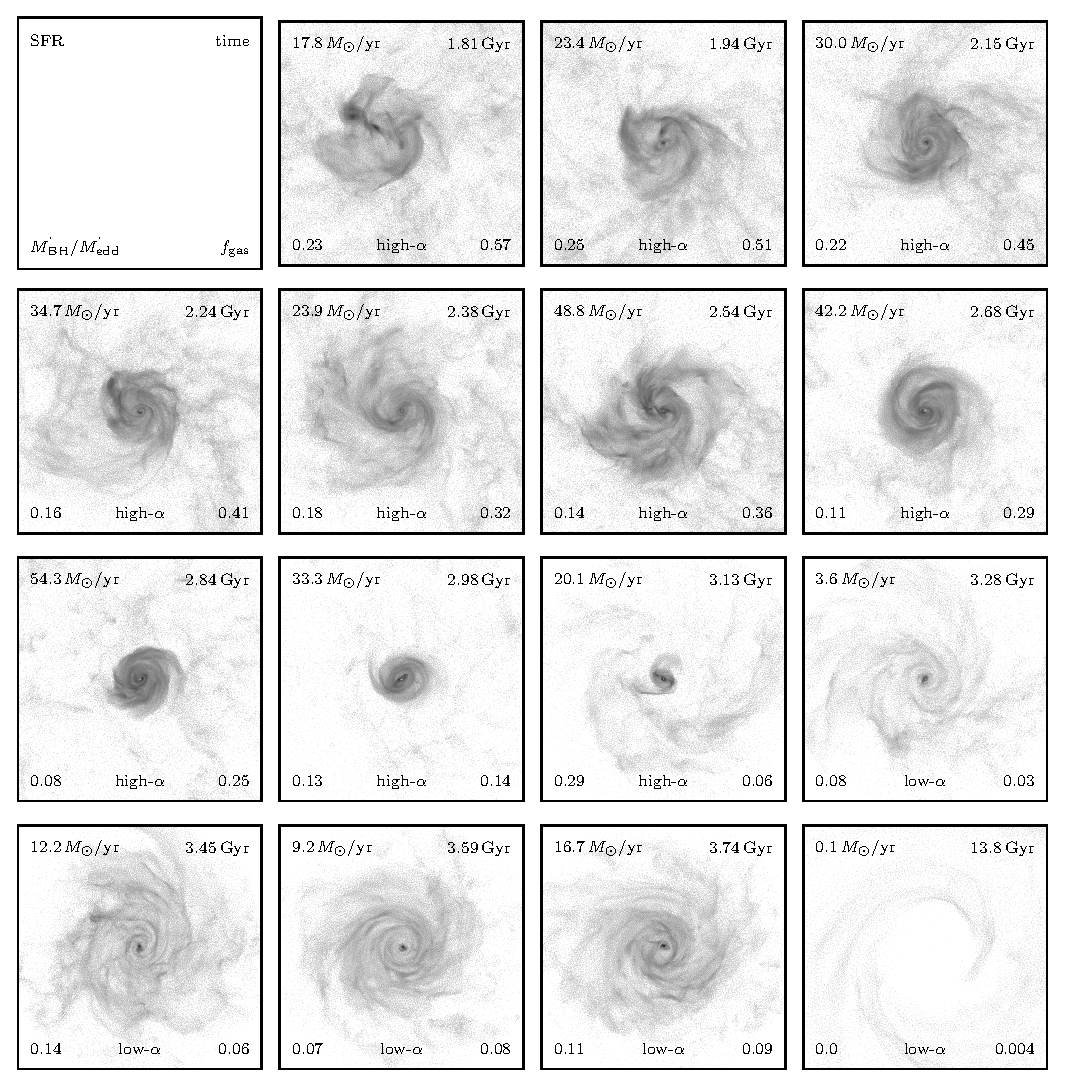
\includegraphics[width=\textwidth]{fig/images_gas.pdf}
  \caption{As in Figure~\ref{fig:images_star}, but showing the surface density projections of gas in our SoI at the transition between the high- and low-$\alpha$ sequences. Each panel indicates subsequent snapshots ranging from snapshot 23 ($z\sim3.5$) to snapshot 36 ($z\sim1.7$), as well as snapshot 99 ($z=0$) in the lower right. Several key numbers are shown in the corners of each panel, clockwise from the top left: SFR, time, gas fraction, and BH accretion rate. A guide is given in the top left subpanel. At the center-bottom of each panel, we indicate panels which occur before the transition ($\sim3.2\,\Gyr$) as high-$\alpha$ and panels which occur after as low-$\alpha$.}
  \label{fig:images_gas}
\end{figure*}

In order to better conceptualize the evolution of the SoI at the high- to low-$\alpha$ transition, we show surface density projections of the stellar (Figure~\ref{fig:images_star}) and gaseous (Figure~\ref{fig:images_gas}) phases of the progenitors of our SoI at various redshifts. In addition to the final, $z=0$, snapshot in the lower right, we show panels for snapshots 23 to 36 in which $z$ ranges from $\sim3.5$ to $\sim1.7$ and the cosmic time from $\sim1.81$ to $\sim3.74\,\Gyr$. Projections are made on a $256\times256$ grid of a $25\,\kpc$ by $25\,\kpc$ square. All star particles/gas cells within ten times the stellar half-mass radius are used, and a simple nearest neighbor assignment of mass to each cell is used. Colors range logarithmically from $5\times10^{-4}$ to $0.5$ in native units ($10^{10} h M_{\odot} \ckpc^{-2}$), and only resolution elements within 10 times the stellar half-mass radius of the center of the subhalo are used.

We also show four relevant statistics in each panel of Figures~\ref{fig:images_star} and \ref{fig:images_gas}. For Figure~\ref{fig:images_star}, these are, clockwise from the upper left, the SFR, cosmic time, bar strength, and BH accretion rate. They are the same for Figure~\ref{fig:images_gas}, but bar strength is replaced with gas fraction (within twice the stellar half-mass radius). The bar strength is missing from several snapshots because the \citet{2022MNRAS.515.1524Z} catalog excludes certain galaxies from being considered barred if they do not pass certain quality cuts. These can come from, e.g., flybys or violent buckling events.

A description of the events portrayed in each Figure is given in Section~\ref{ssec:cause_qui}.

\subsection{One-Zone Model}\label{ssec:onezone}

\begin{figure}
  \centering
  \includegraphics[width=\columnwidth]{fig/mgfe_vice.pdf}
  \caption{\textbf{A higher star formation efficiency leads to a steeper decline in \MgFe{}.} In both panels, the lines show the time evolution of \MgFe{} in a simple one zone chemical evolution model, described in Section~\ref{ssec:onezone_met}. The upper panel shows the evolution of \MgFe{} over $2\,\Gyr$ while the lower panel shows the negative of its time derivative. Decreasing the star formation timescale $\tau_{\star}=M_{\textrm{gas}/\textrm{SFR}}$ leads to a more rapid decline in \MgFe{}. At its steepest decline ($t\sim0.5\,\Gyr$), an order of magnitude decrease in $\tau_{\star}$ leads to a slope nearly a factor of $2$ larger. At later times ($t>1\,\Gyr$), the models with smaller $\tau_{\star}$ reach their steady-state \MgFe{} value more quickly.}
  \label{fig:vice}
\end{figure}

We showed in Figure~\ref{fig:fig1} that a time-linear $\alpha$-enhancement of old stars (forming before $z=1.5$) led to the emergence of a strong chemical bimodality. This $\alpha$-enhancement is equivalent to saying that \alphaFe{} declines more rapdily with time at high-$z$. In Figure~\ref{fig:vice} we demonstrate an argument for why this steeper decline in \alphaFe{} might be absent in TNG.

We show in the upper panel the evolution of \MgFe{} of three one zone chemical evolution models which vary the star formation (SF) timescale. This timescale, $\tau_{\star}$, is the inverse of the SF efficiency. A shorter SF timescale leads to a more rapid reduction in \MgFe{}. In the shortest timescale model, $\tau_{\star}=0.5\,\Gyr$, \MgFe{} drops from $\sim0.45$ to $0.08\,\dex$ in $2\,\Gyr$. In comparison, the longest timescale model, $\tau_{\star}=5\,\Gyr$ only drops to $\sim0.2\,\dex$ in the same time.

The lower panel shows the negative of the time derivative of \MgFe{}. This panel shows the same behavior, with the slope of the $\tau_{\star}=0.5\,\Gyr$ model peaking at $-0.5\,\dex/\Gyr$ compared to the $5\,\Gyr$ model which peaks at $-0.25\,\dex/\Gyr$. After $1\,\Gyr$, the trend starts to reverse, with the longer SF timescale models declining more rapidly, though at a much reduced rate ($\sim-0.1\,\dex/\Gyr$) than at the peak.

\section{Discussion}\label{sec:disc}
In Figure~\ref{fig:fig1}, we compared the abundance plane between the Milky Way and our SoI before and after the $\alpha$-enhancement. It is visibly obvious that the TNG SoI is unimodal before the $\alpha$-enhancement and bimodal afterwards (ignoring the minor mode at high-\MgFe{}). Here, we briefly discuss two main points: (1) assuming the $\alpha$-enhancement is justified, what leads to the bimodality in the SoI?, and (2) what justifies the $\alpha$-enhancement? We then briefly extend our comparison to the Milky Way data.

\subsection{Cause of Bimodality}\label{ssec:bim_cause}
An extensive analysis of our SoI is beyond the scope of this project, but here we argue that the evidence is consistent with the scenario presented in \citet{2024arXiv240707985B}. They presented an idealized simulation resembling the merger between the Milky Way and GSE. They varied the orbital parameters slightly in a grid of 27 simulations and found that simulations which had a brief quiescent period as a result of the merger led to a bimodal abundance distribution. They argued that AGN activity was responsible for this brief quenching.

Once the $\alpha$-enhancement post-processing has been done, the SoI that we have studied in this work is consistent with this scenario. The vertical dashed line in Figures~\ref{fig:alpha} and \ref{fig:history} denotes the transition between the high- and low-$\alpha$ sequences. We place it at an age of $10.6\,\Gyr$ or a formation time of $\sim3.2\,\Gyr$. The upper right panel of Figure~\ref{fig:alpha} shows 2D histograms of \MgFe{} vs star particle age in fixed bins of \FeH{} (each color is a different \FeH{} bin, and an offset is given to \MgFe{} so their medians are at zero). Stars which formed before the dashed line had a steep decline of \MgFe{} with time, while the relation in star particles formed after the dashed line is much more flat. At the line, we see a gap in the $\FeH=-0.5$ and $-0.25$ bins.

The age gap in each \FeH{} bin of Figure~\ref{fig:alpha} is contemperaneous with a minimum in the global SFR. We can see in the upper panel of Figure~\ref{fig:history} that this dashed line lies almost exactly at the point of a local minimum in the SFH. This minimum, which is $\sim3\,\Msunyr$, is 10--15$\times$ smaller than the maxima before and after it.

During this period of suppressed SF, we argue that the relative lack of enrichment of Type~II SNe which leads to a lower rate of Mg production. This leads to a rapid reduction in \MgFe{}. This, combined with a lack of SF in the first place, leads to a scarcity of star particles in the region intermediate between the high- and low-$\alpha$ sequences. A more in-depth explanation is given in Section~4.1 in \citet{2024arXiv240707985B}. 

In the fiducial TNG distribution shown in the upper middle panel of Figure~\ref{fig:alpha}, the same general behavior with respect to the dashed line is present. However, because the \MgFe{} decline before the dashed line is not as strong, star particles which formed before and after the dashed line overlap in the \MgFe{} distribution shown in Figure~\ref{fig:fig1}. 

It is also worth noting that in both the fiducial and $\alpha$-enhanced SoI, there is a sort of rebound effect in \MgFe{}. The star particles which form directly after the dashed line have a slightly lower \MgFe{} than stars which form after. This was seen in Figure~9 of \citet{2024arXiv240707985B}. In that work, it was argued that this occurs because, during the period of suppressed SF, the \alphaFe{} of star forming gas plummets since there is no contribution from Type~II SNe. Later, the \alphaFe{} of the gas will recover when the SFR also recovers, but there is a brief window when old, low-$\alpha$ stars can form.

\subsection{Steepening of $\alpha$ Decline}\label{ssec:sfe}
As described in Section~\ref{ssec:tng}, we applied a post-processing to the \MgFe{} of star particles in the TNG simulation. Specifically, for star particles formed before $z=1.5$, we added to their \MgFe{} a value of $0.1\times\left(t_{1.5}-t_{\textrm{form}}\right)$, where $t_{1.5}$ is the age of the universe at $z=1.5$ ($\sim4.3\,\Gyr$) and $t_{\textrm{form}}$ is the formation time. This post-processed subhalo is presented alongside the fiducial subhalo in the right and middle columns, respectively, of Figures~\ref{fig:fig1} and \ref{fig:alpha}.

The \MgFe{} value of star forming gas is the result of a complicated mixture of many different aspects of the TNG model, to name a few: stellar and AGN feedback which alter gas inflows and outflows, secular, dynamical evolution, SF prescription, magnetic fields, (lack of) cosmic rays, diffusivity of hydrodynamics solver, and, of course, enrichment models. Isolating the cause of the ``incorrect''\footnote{Our case study of a single galaxy, selected in a non-reproducible manner, is hardly cause to firmly assert that the fiducial evolution in TNG50 is incorrect.} \MgFe{} vs time evolution at high-$z$ is not straightforward nor, in our opinion, even possible. However, we do offer one reasonable explanation -- the SFE at high densities, more present at high-$z$, is too low.

We demonstrate the impact of the SFE on the \alphaFe{} ratio using a simple one-zone chemical evolution model with the publicly available code \texttt{VICE}. The details of our setup is given in Section~\ref{ssec:onezone_met}. We vary the SF timescale, $\tau_{\star}=M_{\textrm{gas}}/\textrm{SFR}$, and examine the impact on the \MgFe{} ratio as a function of time. We find that shorter SF timescales do lead to a more rapid reduction in \MgFe{}. The rate of decrease in \MgFe{}, at its maximum, varies from $\sim-0.25\,\dex/\Gyr$ in the $\tau_{\star}=5\,\Gyr$ model to $\sim-0.5\,\dex/\Gyr$ in the $\tau_{\star}=0.5\,\Gyr$ model. For our post-processing, assumed an additional decrease rate of $0.1\,\dex/\Gyr$. Such a difference is well within the range of \MgFe{} decrease seen in our different $\tau_{\star}$ models.

S. Hassan et al. (in preparation) demonstrated that the pressure regulated feedback model of \citet{2022ApJ...936..137O} predicts higher SFRs of patches of gaseous disks in TNG50 than the fiducial model by up to an order of magnitude. This is well within our needed factor of $2$ in $\tau_{\star}$. Therefore, our argument that the \MgFe{} does not decline quickly enough at high-$z$ is reasonably justified. An intuitive understanding of the impact the decline in \alphaFe{} vs time has is that, when \alphaFe{} declines rapidly, it is a better estimator of age. When it is a better estimator of age, events which are separated temporally become better separated in the abundance plane.

\subsection{Comparison to Observations}\label{ssec:compare_obs}
The lower left panel of Figure~\ref{fig:alpha} shows the \MgFe{} vs age of stars in bins of \FeH{} which pass our solar neighborhood selection and are present in the APOKASC2 catalog. In the bins where the bimodality is strongest (blue and orange, $\FeH=-0.5$ and $-0.25$, respectively), we see that there is a sort of two tiered distribution with significant overlap in age. In the SoI with age and abundance errors shown in the lower right panel, a very similar distribution can be seen in all \FeH{} bins. An examination of the true distribution in the SoI (upper right panel), we see that the two distributions are in fact very cleanly separated in age. We do not know the true underlying distribution in the Milky Way, but these panels show that the general picture shown in our SoI is consistent with the Milky Way.

\subsection{Cause of Quiescence}\label{ssec:cause_qui}
% We show the evolution of the SoI in greater detail at the transition between the high- and low-$\alpha$ sequences in Figure~\ref{fig:history_zoom}. As in Figure~\ref{fig:history} we indicate the SFR (blue) and black hole accretion rate (orange), but we also include the strength of the bar, taken to be the maximum value of $A_2$, in red. From $\sim2.8\,\Gyr$ to $\sim3.2\,\Gyr$, the SFR drops from $\sim54\,\Msunyr$ to $3.6\,\Msunyr$. The minimum in the SFR is nearly coincident with the transition line.

% We can see more clearly here that the BH accretion rate (red), in units of the Eddington accretion rate, increases from a value of $\sim0.08$ at $\sim2.8\,\Gyr$ to a maximum of $\sim0.3$ at $\sim3.1\,\Gyr$, right before the transition. This rise in the AGN accretion rate is preceded by a strengthening of the bar, which rises from an $A_2$ of $\sim0.1$ at $t\sim2.4\,\Gyr$ to an $A_2$ of $\sim0.5$ at $\sim3.1\,\Gyr$, the time of the peak BH accretion rate.


It is natural to question why the minimum in the SFR occurs. In \citet{2024arXiv240707985B}, AGN activity from a merger was the suspected cause. Here, we can see that there is indeed a brief burst in AGN accretion at the time of the merger (middle panel of Figure~\ref{fig:history}). Based on this burst, it is reasonable to suspect that AGN activity is also responsible for the quiescent period in our SoI. However, we argue that the cause of the localized spike in the BH accretion rate is not due to a merger but instead due to the formation/strengthening of a bar.

In Figure~\ref{fig:history_zoom}, we take a closer view of the evolution of our SoI at the transition between the high- and low-$\alpha$ sequence, which we denote with the same line at an age of $10.6\,\Gyr$ ($t\sim3.2\,\Gyr$) as before. Here, we see that indeed the drop in the SFR ( $\sim3.6\,\Msunyr$ at $t\sim3.3\,\Gyr$) reaches a minimum one snapshot after the maximum in the BH accretion rate ($\sim0.3\times\dot{M_{\textrm{edd}}}$ at $t\sim3.1\,\Gyr$).

The gaseous surface density images in Figure~\ref{fig:images_gas} are helpful to understand this moment in the SoI's history. The third row, from $t=2.84$ to $3.28\,\Gyr$ shows this moment, with the rightmost $t=3.28\,\Gyr$ marking the transition from high- to low-$\alpha$ formation. The gas fraction (bottom right number) quickly drops from $25\%$ to $3\%$, accompanied by not only a high SFR ($54.3\,\Msunyr$ at maximum) but also an increasing BH accretion rate.

This increasing BH accretion rate is also preceded by the formation of a stellar bar at the center of the galaxy as seen in Figure~\ref{fig:images_star}.\footnote{The bar is already at a strength of $\Atmax\sim0.1$ before, so it either forms or strengthens depending on one's interpretation. We choose the former.} Starting from $t=2.38\,\Gyr$, the bar strength grows from $\Atmax=0.1$ to $0.5$ at $t=3.13\,\Gyr$, the peak of the BH accretion rate. Note that the bar strength considers only the region where the phase of the second Fourier mode is constant, and so spiral structure as seen in, e.g., the $t=2.38\,\Gyr$ snapshot is not eligible for \Atmax{}.

The scenario implied by all the available evidence is that: 
\begin{enumerate}
  \item a bar forms through an internal instability, which
  \item drives a large amount of gas to the center of the galaxy, which
  \item triggers a high BH accretion rate and quasar-mode thermal feedback, which
  \item clears gas out of the galaxy.
\end{enumerate}
This picture is supported by work showing that in simulations bars should be able to fuel AGN \citep{1990Natur.345..679S,2010MNRAS.407.1529H}, and that barred galaxies preferentially host AGN \citep{2022A&A...661A.105S}. At high-$z$, the AGN mechanism is thought to be responsible for quenching \citep[e.g.][and references therein]{2023arXiv230806317D,2024arXiv240417945P,2024arXiv240518685M,2024Natur.630...54B}.

A complicating factor for this picture comes from the high SFR associated with the galaxy. The depletion time ($M_{\textrm{gas}}/\textrm{SFR}$) at the $t=2.84\,\Gyr$ snapshot is $204\,\Myr$, shorter than the time it takes for the SFR to reach its minimum. However, this has to be balanced by the fact that the depletion time is already short at this redshift. The average depletion time in the preceding 5 snapshots is $220\,\Myr$, so clearly the SoI is accreting high amounts of gas from its CGM. A definitive account, difficult with the current simulation because of its sparse snapshot spacing, requires further work.

% \subsection{Full Sample}\label{ssec:fullsamp}

\section{Conclusions}\label{sec:conc}
In this work, we examined a specific subhalo in Illustris TNG50. This subhalo is at a Milky Way-progenitor mass at high-$z$ ($z\sim2$). After applying a post-processing step that increased the \MgFe{} of star particles formed before $z=1.5$, this subhalo hosts a strong bimodality in the plane of \MgFe{} and \FeH{}, shown in Figure~\ref{fig:fig1}. This post-processing is justified by arguing that the SFE of dense gas is too low in TNG (Section~\ref{ssec:sfe}).

This bimodality can be traced to an event that occurred at an age of $10.6\,\Gyr$, or formation time of $\sim3.2\,\Gyr$ ($z\sim2$). Shown as a vertical dashed line in Figure~\ref{fig:alpha}, star particles which form before this form at high-$\alpha$ while stars which form after form at lower $\alpha$. At the dashed line, there is a gap. We argue that the presence of this gap is responsible for the valley in the bimodality (Figure~\ref{fig:fig1}). It is accompanied by a global reduction in the SFR by about a factor of 6 (upper panel of Figure~\ref{fig:history}).

The reduction in the SFR has two effects. First, a lower production of Mg is the natural result of a lack of Type~II SNe. Second, the lack of SF means that stars at \MgFe{} intermediate between the high- and low-$\alpha$ sequences never form. This is the same argument that was first presented in \citet{2024arXiv240707985B}. When observational errors are added to the subhalo's abundance vs age distribution, we show that it is broadly consistent with the Milky Way's abundance-age distribution (Section~\ref{ssec:compare_obs}).

While a strong claim about the cause of the quiescent period is difficult to make, we showed that the formation/strengthening of a bar could be responsible for triggering an episode of AGN activity. This work adds further support that the argument made in \citet{2024arXiv240707985B} is a plausible explanation for the Milky Way's abundance bimodality.

\begin{acknowledgements}
This work has made use of data from the European Space Agency (ESA) mission {\it Gaia} (\url{https://www.cosmos.esa.int/gaia}), processed by the {\it Gaia} Data Processing and Analysis Consortium (DPAC, \url{https://www.cosmos.esa.int/web/gaia/dpac/consortium}). Funding for the DPAC has been provided by national institutions, in particular the institutions participating in the {\it Gaia} Multilateral Agreement.
\end{acknowledgements}

\bibliography{ref}{}
\bibliographystyle{aasjournal}

\appendix

\section{Observational Errors}\label{app:obs_err}
In Figure~\ref{fig:alpha}, we assumed observational errors of $15\%$ in age and $0.01\,\dex$ in \MgFe{}. In Figure~\ref{fig:obs_err}, we plot the quoted observational errors of the APOKASC2 (left) and ASPCAP (right) datasets, showing both \FeH{} and \MgFe{} (blue and orange, respectively). We show our $15\%$ age error and $0.01\,\dex$ abundance error assumptions as black lines. For the age error, we used the maximum of the upper and lower estimates from \citet{2018ApJS..239...32P}. Our assumed errors are generally consistent with the errors. Our error in \MgFe{} is a bit smaller than in ASPCAP, but the age estimates are by far the more constraining of the two.

\begin{figure*}
  \centering
  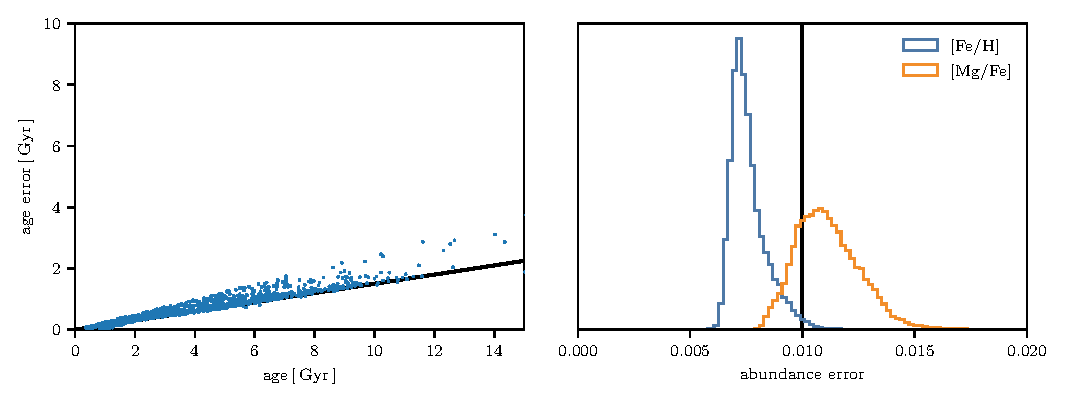
\includegraphics[width=\columnwidth]{fig/obs_error.pdf}
  \caption{The observational errors of the APOKASC2 (left) and ASPCAP dataset (right). We show, on the left, a line indicating a $15\%$ error in observed age and on the right a vertical line indicating a $0.01\,\dex$ error.}
  \label{fig:obs_err}
\end{figure*}

\section{Random Selection of Subhalos}\label{app:rand_fig1}
In Figures~\ref{fig:app0} to \ref{fig:app16}, we show a version of Figure~\ref{fig:fig1} but for a random selection of subhalos from our broader sample of 168 Milky Way-progenitors at $z=1.5$ in TNG50. It is from this sample that we selected our SoI. We first show our SoI at $z=1.5$ in Figure~\ref{fig:app0}, and then show our random sample of 16.

\begin{figure*}
  \centering
  \includegraphics[width=\textwidth]{fig/app_172175.pdf}
  \caption{The same as Figure~\ref{fig:fig1}, but for our SoI at $z=1.5$.}
  \label{fig:app0}
\end{figure*}

\begin{figure*}
  \centering
  \includegraphics[width=\textwidth]{fig/app_163071.pdf}
  \caption{The same as Figure~\ref{fig:fig1}, but for a random subhalo from our catalog at $z=1.5$.}
  \label{fig:app1}
\end{figure*}

\begin{figure*}
  \centering
  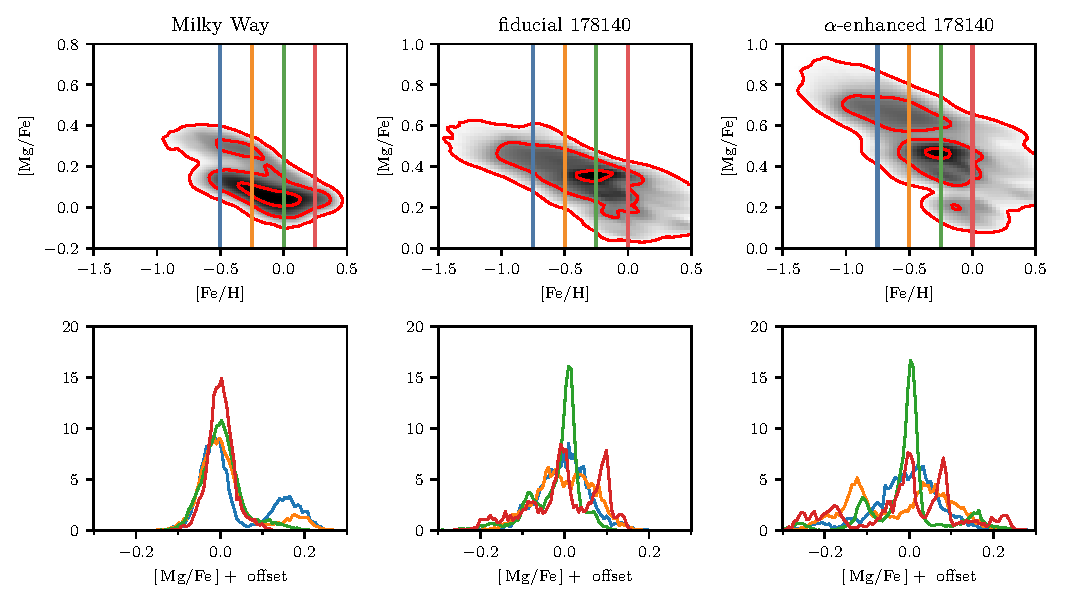
\includegraphics[width=\textwidth]{fig/app_178140.pdf}
  \caption{The same as Figure~\ref{fig:fig1}, but for a random subhalo from our catalog at $z=1.5$.}
  \label{fig:app2}
\end{figure*}

\begin{figure*}
  \centering
  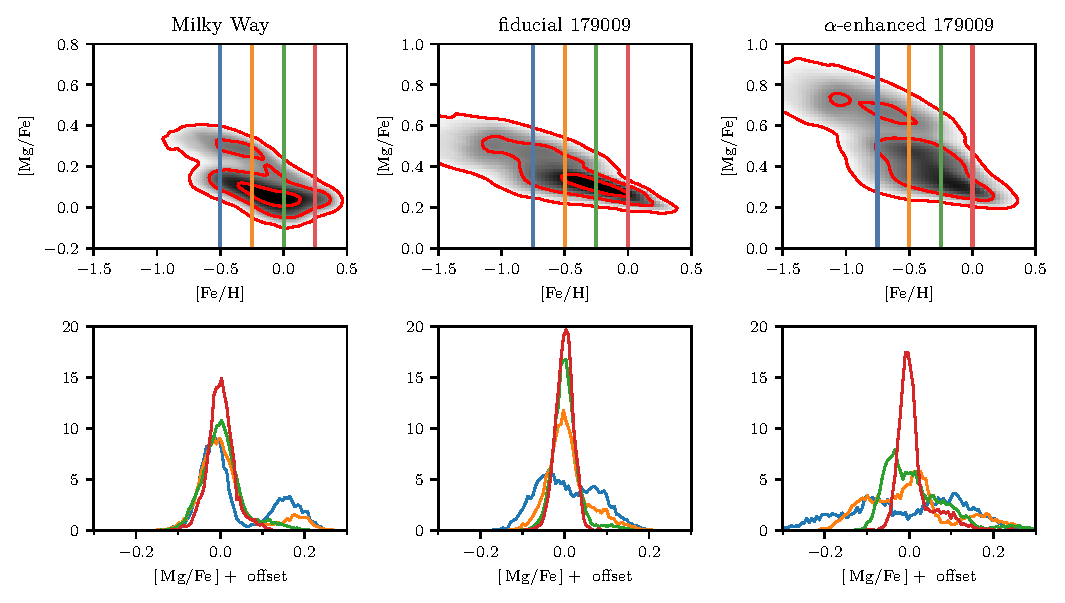
\includegraphics[width=\textwidth]{fig/app_179009.pdf}
  \caption{The same as Figure~\ref{fig:fig1}, but for a random subhalo from our catalog at $z=1.5$.}
  \label{fig:app3}
\end{figure*}

\begin{figure*}
  \centering
  \includegraphics[width=\textwidth]{fig/app_193025.pdf}
  \caption{The same as Figure~\ref{fig:fig1}, but for a random subhalo from our catalog at $z=1.5$.}
  \label{fig:app4}
\end{figure*}

\begin{figure*}
  \centering
  \includegraphics[width=\textwidth]{fig/app_196834.pdf}
  \caption{The same as Figure~\ref{fig:fig1}, but for a random subhalo from our catalog at $z=1.5$.}
  \label{fig:app5}
\end{figure*}

\begin{figure*}
  \centering
  \includegraphics[width=\textwidth]{fig/app_202467.pdf}
  \caption{The same as Figure~\ref{fig:fig1}, but for a random subhalo from our catalog at $z=1.5$.}
  \label{fig:app6}
\end{figure*}

\begin{figure*}
  \centering
  \includegraphics[width=\textwidth]{fig/app_208267.pdf}
  \caption{The same as Figure~\ref{fig:fig1}, but for a random subhalo from our catalog at $z=1.5$.}
  \label{fig:app7}
\end{figure*}

\begin{figure*}
  \centering
  \includegraphics[width=\textwidth]{fig/app_222555.pdf}
  \caption{The same as Figure~\ref{fig:fig1}, but for a random subhalo from our catalog at $z=1.5$.}
  \label{fig:app8}
\end{figure*}

\begin{figure*}
  \centering
  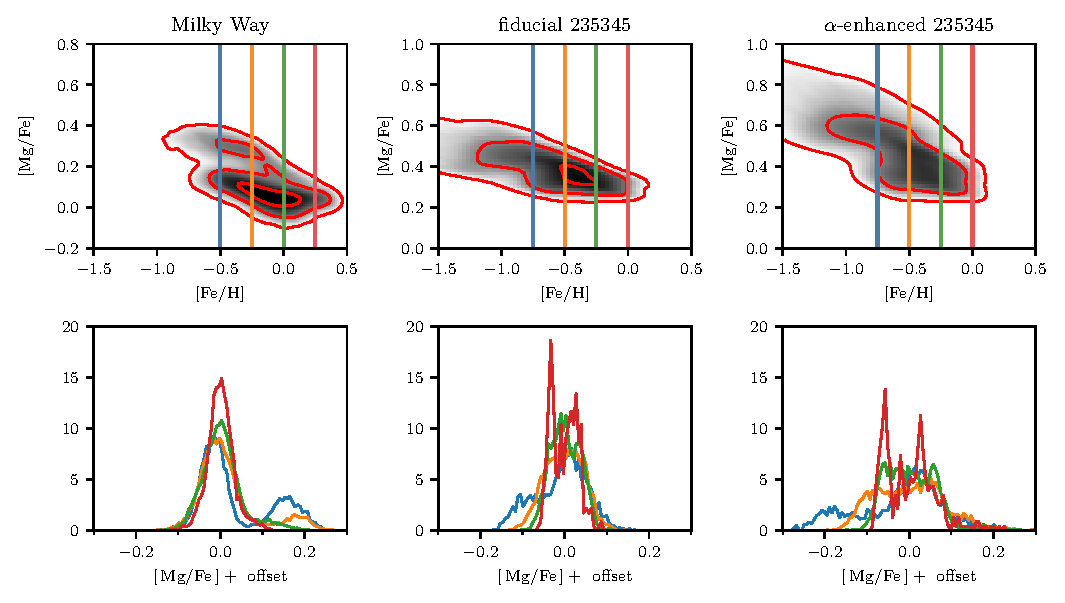
\includegraphics[width=\textwidth]{fig/app_235345.pdf}
  \caption{The same as Figure~\ref{fig:fig1}, but for a random subhalo from our catalog at $z=1.5$.}
  \label{fig:app9}
\end{figure*}

\begin{figure*}
  \centering
  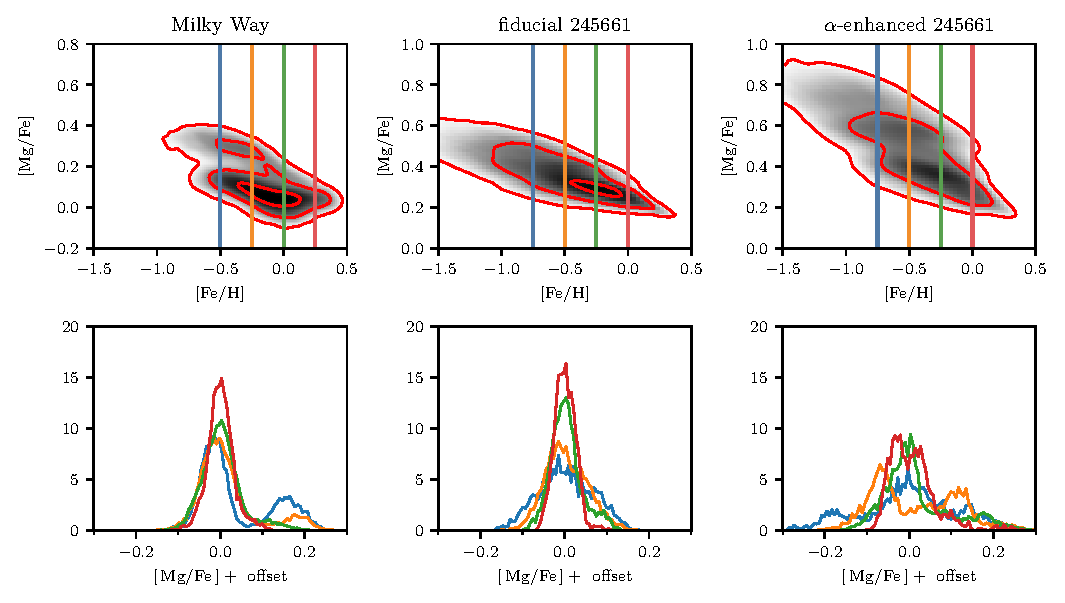
\includegraphics[width=\textwidth]{fig/app_245661.pdf}
  \caption{The same as Figure~\ref{fig:fig1}, but for a random subhalo from our catalog at $z=1.5$.}
  \label{fig:app10}
\end{figure*}

\begin{figure*}
  \centering
  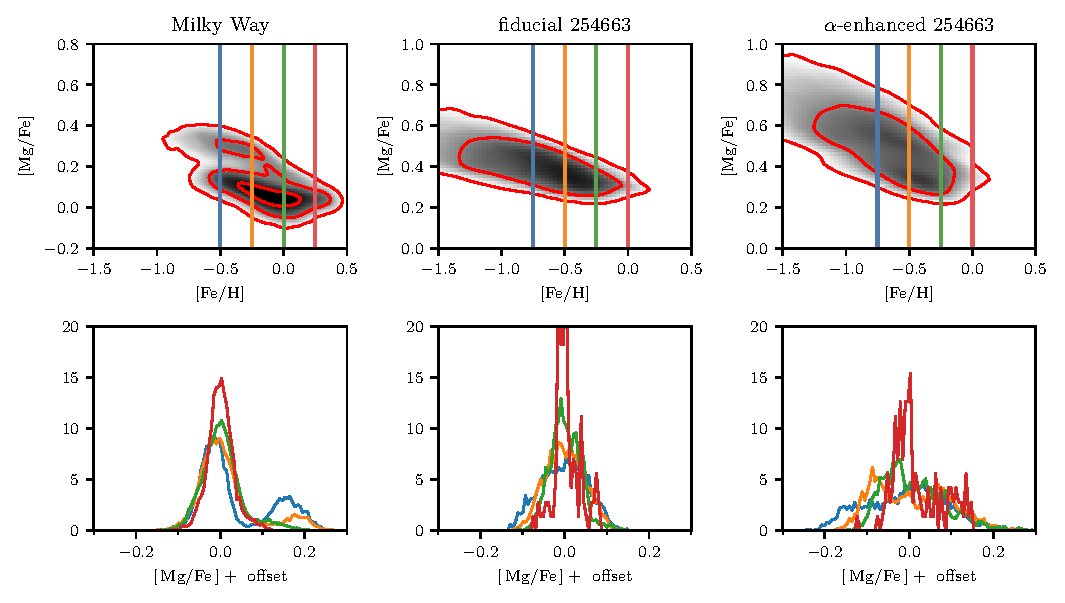
\includegraphics[width=\textwidth]{fig/app_254663.pdf}
  \caption{The same as Figure~\ref{fig:fig1}, but for a random subhalo from our catalog at $z=1.5$.}
  \label{fig:app11}
\end{figure*}

\begin{figure*}
  \centering
  \includegraphics[width=\textwidth]{fig/app_260347.pdf}
  \caption{The same as Figure~\ref{fig:fig1}, but for a random subhalo from our catalog at $z=1.5$.}
  \label{fig:app12}
\end{figure*}

\begin{figure*}
  \centering
  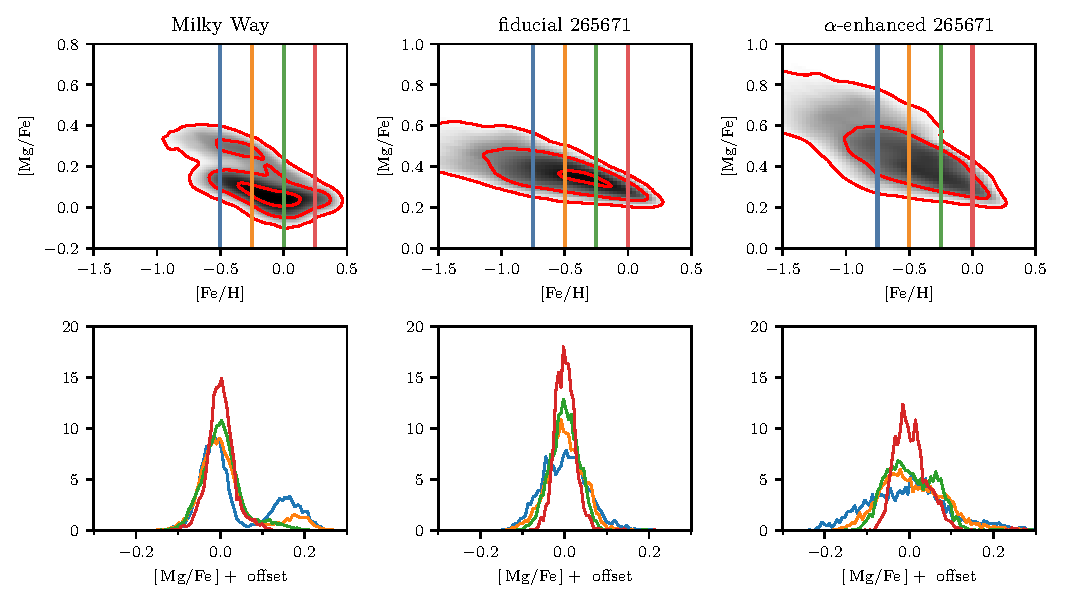
\includegraphics[width=\textwidth]{fig/app_265671.pdf}
  \caption{The same as Figure~\ref{fig:fig1}, but for a random subhalo from our catalog at $z=1.5$.}
  \label{fig:app13}
\end{figure*}

\begin{figure*}
  \centering
  \includegraphics[width=\textwidth]{fig/app_282632.pdf}
  \caption{The same as Figure~\ref{fig:fig1}, but for a random subhalo from our catalog at $z=1.5$.}
  \label{fig:app14}
\end{figure*}

\begin{figure*}
  \centering
  \includegraphics[width=\textwidth]{fig/app_287601.pdf}
  \caption{The same as Figure~\ref{fig:fig1}, but for a random subhalo from our catalog at $z=1.5$.}
  \label{fig:app15}
\end{figure*}

\begin{figure*}
  \centering
  \includegraphics[width=\textwidth]{fig/app_292983.pdf}
  \caption{The same as Figure~\ref{fig:fig1}, but for a random subhalo from our catalog at $z=1.5$.}
  \label{fig:app16}
\end{figure*}

\end{document}
